\subsection{Problema de programação linear}

Utilizando algumas aproximações, o problema de programação não linear inteiro misto pode ser convertido em um problema de programação linear inteiro misto.

Inicialmente pode-se aproximar o quadrado da tensão em um nó do circuito como o quadrado da tensão nominal.
Esta simplificação é valida e com um erro de aproximação baixo, devido ao intervalo restrito da magnitude de tensão [$\underline{V}^2$,$\overline{V}^2$] e comprovado experimentalmente depois de realizar varias simulações apresentadas em~\cite{Goncalves2013ModelosRadiais} e \cite{Alves2012Alocacao-}.
Dessa forma o primeiro termo da equação~\eqref{eq:PNLIM_power} pode ser reescrita da seguinte forma:

\begin{equation}\label{eq:L_powervoltage}
    V_{j}^{2}I_{ij}^{sqr} \approx (V^{\text{nom}})^{2}I_{ij}^{sqr}\qquad\forall ij\in\Omega_{l}
\end{equation}

Da equação~\eqref{eq:L_powervoltage}, é possível perceber que não existe mais produto entre variáveis, visto que $V^{nom}$ é um parâmetro e, portanto, uma constante do problema.

O outro passo é linearizar os termos $P_{ij}^2$ e $Q_{ij}^2$, o que é possível, utilizando o método de linearização por partes como mostrado em~\cite{Goncalves2013ModelosRadiais} e \cite{Alves2012Alocacao-}.

O método de linearização por partes consiste em uma somatória de segmentos de retas a partir de blocos discretos igualmente espaçados.
A figura~\ref{fig:linearization} mostra a discretização do módulo de uma variável pelo seu quadrado.

\begin{figure}[H]
    \centering
    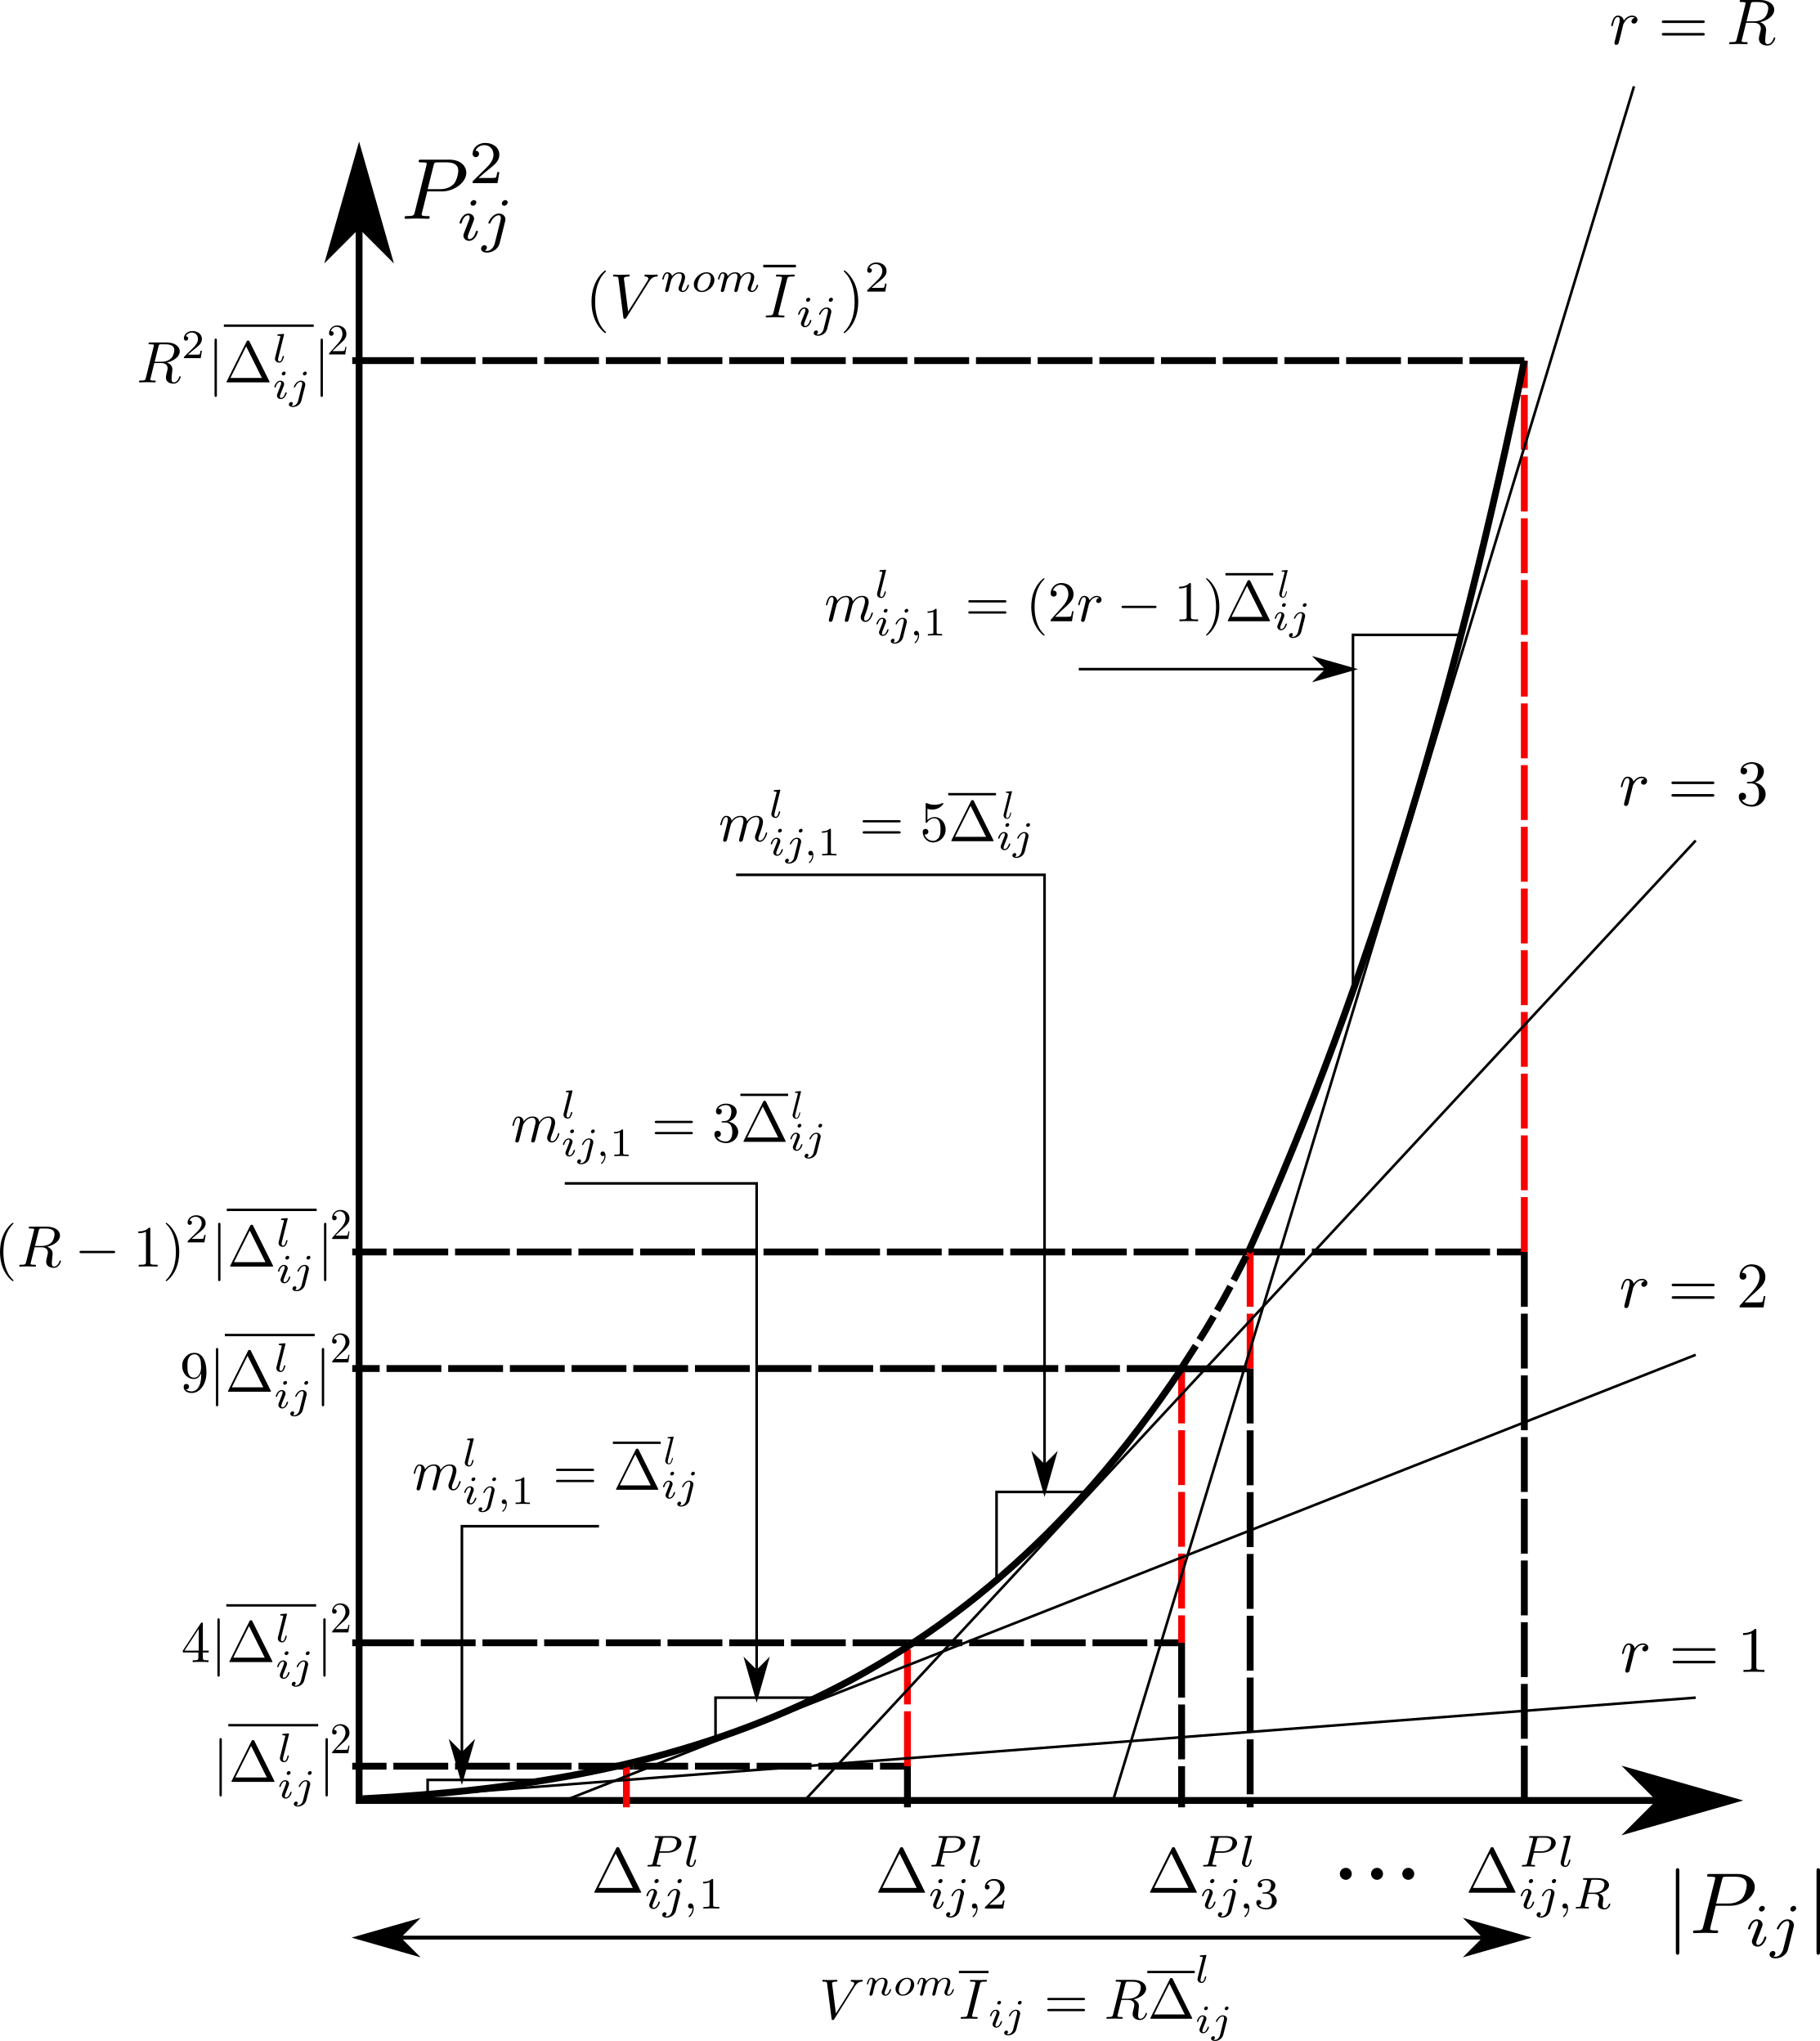
\includegraphics[width = 0.6\textwidth]{5_Formulation/lin.png}
    \caption{Linearização da potência ativa pelo método de linearização por partes}
    \label{fig:linearization}
\end{figure}{}

Com base na figura~\ref{fig:linearization}, o valor de $P_{ij}^{2}$ pode ser descrito como o somatório dos catetos paralelos ao eixo da ordenada (segmentos em vermelho), a mesma analogia pode ser feita com $Q_{ij}^{2}$, resultando na equação~\eqref{eq:Lin_quadpower}.

\begin{equation}\label{eq:Lin_quadpower}
    P_{ij}^2 + Q_{ij}^2 \approx \sum_{r = 1}^{R}m_{ij,r}^{l}\Delta_{ij,r}^{Pl} + \sum_{r = 1}^{R}m_{ij,r}^{l}\Delta_{ij,r}^{Ql} \qquad\forall ij\in\Omega_{l} 
\end{equation}

Tal que $\Delta_{ij,r}^{Pl}$ e $\Delta_{ij,r}^{Ql}$ são variáveis que representam o r-ésimo bloco de $P_{ij}$ e $Q_{ij}$ do circuito $ij$ respectivamente, as quais devem obedecer a seguinte restrição:

\begin{equation}\label{eq:Lin_Pdeltalim}
    0 \leq \Delta_{ij,r}^{Pl} \leq \overline{\Delta}_{ij,r}^l \qquad\forall ij\in\Omega_{l} 
\end{equation}

\begin{equation}\label{eq:Lin_Qdeltalim}
    0 \leq \Delta_{ij,r}^{Ql} \leq \overline{\Delta}_{ij,r}^l \qquad\forall ij\in\Omega_{l} 
\end{equation}

O parâmetro $\Delta_{ij}^{l}$ representa o valor máximo do bloco de discretização, assim dado um valor $R$ de discretizações, pode-se determinar $\Delta_{ij}^{l}$ como o quociente entre o módulo da potência aparente máxima e a quantidade de discretizações $R$, obtendo assim a equação~\eqref{eq:Lin_maxdelta}.

\begin{equation}\label{eq:Lin_maxdelta}
    \overline{\Delta}_{ij}^{l} = \frac{V^{\text{nom}}\overline{I}_{ij}}{R} \qquad\forall ij\in\Omega_{l} 
\end{equation}

$m_{ij,r}^{l}$ representa a inclinação do r-ésimo bloco de potência ativa e reativa no circuito $ij$ e é descrito pela equação~\eqref{eq:Lin_m}.

\begin{equation}\label{eq:Lin_m}
    \begin{split}
        m_{ij,r}^{l} & = \frac{r^2|\overline{\Delta_{ij}^{l}}|^2 - (r-1)^2|\overline{\Delta_{ij}^{l}}|^2}{|\overline{\Delta_{ij}^{l}}|}\qquad\forall ij\in\Omega_{l}\\
        & = |\overline{\Delta_{ij}^{l}}|(r^2 - r^2 + 2r - 1)\qquad\quad\forall ij\in\Omega_{l}\\
        & = (2r-1)\overline{\Delta_{ij}^{l}}\qquad\qquad\qquad\qquad\forall ij\in\Omega_{l}
    \end{split}
\end{equation}

Para que se possa implementar a linearização descrita pelas equações anteriores é preciso modelar o módulo das variáveis $P_{ij}$ e $Q_{ij}$. Isto pode ser feito utilizando duas variáveis positivas de tal modo que:

\begin{equation}\label{eq:Lin_PQmod}
    \begin{split}
        P_{ij} = P_{ij}^{+} - P_{ij}^{-} & \qquad\forall ij\in\Omega_{l}\\
        Q_{ij} = Q_{ij}^{+} - Q_{ij}^{-} & \qquad\forall ij\in\Omega_{l}
    \end{split}
\end{equation}

\begin{equation}
    \begin{split}
        0 \leq P_{ij}^{+} & \qquad\forall ij\in\Omega_{l}\\
        0 \leq P_{ij}^{-} & \qquad\forall ij\in\Omega_{l}\\
        0 \leq Q_{ij}^{+} & \qquad\forall ij\in\Omega_{l}\\
        0 \leq Q_{ij}^{-} & \qquad\forall ij\in\Omega_{l}
    \end{split}
\end{equation}

Aplicando o módulo em $P_{ij}$ e $Q_{ij}$, obtém-se:

\begin{equation}\label{eq:Lin_modPA}
        |P_{ij}| = P_{ij}^{+} + P_{ij}^{-} = \sum_{r = 1}^{R}\Delta_{ij,r}^{Pl}  \qquad\forall ij\in\Omega_{l}
\end{equation}

\begin{equation}\label{eq:Lin_modPR}
        |Q_{ij}| = Q_{ij}^{+} + Q_{ij}^{-} = \sum_{r = 1}^{R}\Delta_{ij,r}^{Ql}  \qquad\forall ij\in\Omega_{l}
\end{equation}

Por fim, o problema de programação linear inteiro misto pode ser descrito no seguinte formato:


\begin{tcolorbox}[breakable,pad at break*=1mm,colback=white!10,title =\textbf{Problema de PLIM para RSD}]

\begin{equation}\label{eq:plim}
\left.
    \begin{tabular}{ll}
               & Min ~\eqref{eq:PNLIM_funcobj}\\
    Sujeito a: &\eqref{eq:PNLIM_fluxoP} - \eqref{eq:PNLIM_voltage}, \eqref{eq:PNLIM_voltagekeys} - \eqref{eq:PNLIM_currentlim} \textbf{(Equações já propostas para RSD)}\\
    &\textbf{(Bloco de equações para linearização de~\eqref{eq:PNLIM_power})}\\
    &$(V^{nom})^{2}I_{ij}^{sqr} = \sum_{r = 1}^{R}m_{ij,r}^{l}\Delta_{ij,r}^{Pl} + \sum_{r = 1}^{R}m_{ij,r}^{l}\Delta_{ij,r}^{Ql} \qquad\forall ij\in\Omega_{l}$ \\
    &$P_{ij} = P_{ij}^{+} - P_{ij}^{-}\qquad\forall ij\in\Omega_{l}$\\
    &$Q_{ij} = Q_{ij}^{+} - Q_{ij}^{-}\qquad\forall ij\in\Omega_{l}$\\
    & $P_{ij}^{+} + P_{ij}^{-} = \sum_{r = 1}^{R}\Delta_{ij,r}^{Pl}  \qquad\forall ij\in\Omega_{l}$\\
    & $Q_{ij}^{+} + Q_{ij}^{-} = \sum_{r = 1}^{R}\Delta_{ij,r}^{Ql}  \qquad\forall ij\in\Omega_{l}$\\
    & $0 \leq \Delta_{ij,r}^{Pl} \leq \overline{\Delta}_{ij,r}^l \qquad\forall ij\in\Omega_{l}$\\
    & $0 \leq \Delta_{ij,r}^{Ql} \leq \overline{\Delta}_{ij,r}^l \qquad\forall ij\in\Omega_{l}$\\
    &$P_{ij}^{+}\in\mathbb{R}^{+}$, $P_{ij}^{-}\in\mathbb{R}^{+}$, $Q_{ij}^{+}\in\mathbb{R}^{+}$, $Q_{ij}^{-}\in\mathbb{R}^{+}\qquad\forall ij\in\Omega_{l}$\\
    & \textbf{(Definição de variáveis binárias)}\\
    &$w_{ij}\in\{0,1\}\qquad\forall ij\in\Omega_{l}$\\
    &\\
    Em que:&\\
    & $m_{ij,r}^{l}= (2r-1)\overline{\Delta_{ij}^{l}}\qquad\qquad\qquad\qquad\forall ij\in\Omega_{l} $\\
    & $\overline{\Delta}_{ij}^{l} = \frac{V^{\text{nom}}\overline{I}_{ij}}{R} \qquad\forall ij\in\Omega_{l}$
    \end{tabular}
\right \}
\end{equation} 
\end{tcolorbox}


